\documentclass[11pt,a4paper]{amsart}
\usepackage{amssymb,amsthm,mathtools}
\usepackage[no-math]{fontspec}
\setmonofont{DejaVuSansMono.ttf}[Scale=0.82]
\usepackage[margin=27mm]{geometry}
\usepackage{booktabs}
\usepackage{tikz}
\usepackage{enumitem}
\usepackage[colorlinks=true,linkcolor=blue!50!black,urlcolor=blue!50!black,citecolor=blue!50!black]{hyperref}

\newtheorem{theorem}{Theorem}
\newtheorem{lemma}[theorem]{Lemma}
\newtheorem{proposition}[theorem]{Proposition}
\newtheorem{corollary}[theorem]{Corollary}
\theoremstyle{definition}
\newtheorem{definition}[theorem]{Definition}
\theoremstyle{remark}
\newtheorem{remark}[theorem]{Remark}

\newcommand{\N}{\mathbb{N}}
\newcommand{\Z}{\mathbb{Z}}
\newcommand{\U}{\mathrm{U}}
\newcommand{\D}{\mathrm{D}}
\newcommand{\lean}[1]{\texttt{#1}}
\newcommand{\len}[1]{\lvert #1\rvert}
\newcommand{\paperdate}{10 November 2026}
\newcommand{\searchdate}{10 November 2026}

\title[Maximal halting times of Wolfram's 2-state 2-symbol Turing machines]{A machine-checked proof of Hasler's conjecture on the maximal halting times of Wolfram's 2-state 2-symbol Turing machines (OEIS A393317)}

\author{Claude Fable 5}
\thanks{Claude Fable 5 is an AI model made by Anthropic (model ID \texttt{claude-fable-5-2}).
The work was commissioned by Dr.\ Marc Potempa; see the statement on authorship and status in
Section~\ref{sec:status}. Lean sources: \url{https://github.com/MarcPotempa/a393317-lean-proof}}
\date{\paperdate}

\begin{document}

\begin{abstract}
For $n\ge 1$ let $a(n)$ be the largest halting time of any of the $4096$ Turing machines with two states and
two symbols, in the one-sided set-up of Wolfram, over all inputs with $n$ binary digits (OEIS A393317).
M.~F.~Hasler conjectured in February 2026 that $a(n)=2(n+2)^2-1$ for $n<5$ and $a(n)=2^{n+2}-3$ for $n>4$,
and that these values are the maximal halting times of machine $1447$ and of machines $378$ and $1351$,
respectively, attained for the input $2^n-1$. We prove the conjecture. The proof is formalized in
Lean~4 with Mathlib and checked by the Lean kernel. The lower bound comes from an exact analysis of three
machines. The upper bound for all $4096$ machines uses crossing sequences at the cell boundaries: for $4092$
machines a small certificate (a finite automaton on crossing sequences, two invariants and a potential
function) is found by a search program and verified by a checker that is proved correct in Lean; the remaining
four machines are treated by hand.
\end{abstract}

\maketitle

\section{Introduction and result}

In a study of the difficulty of computation \cite{wolfram}, S.~Wolfram enumerates the $4096$ Turing machines
with two states and two symbols and runs each of them on the binary digits of an integer, with the convention
that the machine halts as soon as the head leaves the tape on the right of its starting cell. Among other
things he records the longest running times and notes that they are dominated by machines $378$ and $1351$.
The corresponding sequence was entered into the OEIS as A393317 by S.~A.~Irvine on 10 February 2026
\cite{oeis}; it reads
\[
17,\ 31,\ 49,\ 71,\ 125,\ 253,\ 509,\ 1021,\ 2045,\ \dots
\]
with $18$ terms known by exhaustive computation (the last six due to R.~P.~P.~McKone). On 12 February 2026
M.~F.~Hasler added a conjecture to the entry, which in our words reads as follows.

\begin{quote}
The maximal runtime of machines $378$ and $1351$ is $2^{n+2}-3$, attained for the $n$-bit input $2^n-1$, while
for machine $1447$ it is $2(n+2)^2-1$, for the same input. Moreover $a(n)=2(n+2)^2-1$ for $n<5$ and
$a(n)=2^{n+2}-3$ for $n>4$.
\end{quote}

The precise model is given in Section~\ref{sec:model}. Write $T_m(x)$ for the halting time of machine $m$ on
the input $x$ if the machine halts, and call $x$ an \emph{$n$-bit input} if $2^{n-1}\le x<2^n$.

\begin{theorem}[Hasler's conjecture]\label{thm:main}
For every $n\ge1$,
\[
\max\bigl\{\,T_m(x) : 0\le m<4096,\ 2^{n-1}\le x<2^n,\ m \text{ halts on } x \,\bigr\}
=\begin{cases} 2(n+2)^2-1 & \text{if } n<5,\\ 2^{n+2}-3 & \text{if } n\ge5.\end{cases}
\]
The same holds if all inputs $0\le x<2^n$ are admitted.
\end{theorem}

\begin{theorem}\label{thm:single}
Let $n\ge1$.
\begin{enumerate}[label=\textup{(\alph*)},leftmargin=2em]
\item Machines $378$ and $1351$ halt on every input. If the binary expansion of $x$ ends in exactly $k$ ones,
both halt after exactly $2^{k+2}-3$ steps. In particular their maximal halting time over the $n$-bit inputs
is $2^{n+2}-3$, attained exactly for $x=2^n-1$.
\item Machine $1447$ halts on the input $2^n-1$ after exactly $2(n+2)^2-1$ steps, and this is its maximal
halting time over the $n$-bit inputs.
\end{enumerate}
\end{theorem}

Both theorems are formalized in Lean~4 \cite{lean4} with Mathlib \cite{mathlib}; the formal statements are
reproduced in Section~\ref{sec:formal}. The proof uses no axioms beyond the three standard ones of Lean
(\lean{propext}, \lean{Quot.sound}, \lean{Classical.choice}) and neither \lean{sorry} nor
\lean{native\_decide}.

\subsection*{Idea of the proof}
The lower bound is elementary: machines $378$ and $1351$ are binary counters, machine $1447$ sweeps back and
forth over a growing block (Section~\ref{sec:lower}). The work is in the upper bound, which is a statement
about all $4096$ machines and all inputs, including the many machines that do not halt on some inputs.
Since the tape is bounded on the right, a halting run can be cut along the cell boundaries. For each boundary
we record a \emph{crossing sequence}, a classical device (see Hennie~\cite{hennie}): here, the list of pairs (state
in which the head crosses to the left, state in which it comes back). The halting time is twice the total
length of these lists minus one, and neighbouring lists are coupled by a relation that involves only the one
cell between them (Section~\ref{sec:crossing}). This turns the question into a combinatorial one about chains
of lists $h_0\to h_1\to h_2\to\cdots$. For a given machine, a finite automaton reading these lists, together
with two invariants and a potential function, bounds the total length (Section~\ref{sec:cert}). Such
certificates are found by a program and checked in Lean, in the spirit of the deciders used for the fifth
busy beaver value \cite{bb5}. Four machines have crossing sequences that the automata cannot control; they
are analysed directly (Section~\ref{sec:special}).

\subsection*{Related work}
As far as we could determine by searches on \searchdate\ (OEIS, GitHub, arXiv, Zenodo, general web search), no
proof of the conjecture had been published. A related statement about a single machine, P.~Bala's formula
$2^{v_2(n)+2}-3$ for the halting time of machine $3626$ on the input $n$ (OEIS A393210), was formalized in
November 2026 in the project \cite{trureturing}.

\section{The model}\label{sec:model}

The tape consists of cells numbered $0,1,2,\dots$; each holds a symbol $0$ or $1$. For the input $x$, cell $i$
initially holds the binary digit of $x$ of weight $2^i$. ``Right'' means towards cell $0$, ``left'' towards
higher cells; so the tape is infinite to the left and ends on the right with cell $0$. The machine has two
states, $\U$ (the start state) and $\D$. The head starts on cell $0$ in state $\U$. In each step the machine
reads the symbol under the head, writes a symbol, changes its state and moves one cell to the left or right.
The machine \emph{halts} with the step in which the head moves right from cell $0$. The \emph{halting time}
is the number of steps performed, this last one included.

The machine number $m\in\{0,\dots,4095\}$ is read as four digits in base $8$,
$m=512\,d_{\U1}+64\,d_{\U0}+8\,d_{\D1}+d_{\D0}$, one for each combination of state and scanned symbol. A digit
$d$ means: the new state is $\U$ if $d<4$ and $\D$ otherwise; the symbol written is $\lfloor d/2\rfloor \bmod 2$;
the head moves right if $d$ is odd and left if $d$ is even. We write a rule as, e.g., $\U1\to\U0\mathrm{L}$
(in state $\U$ on symbol $1$: write $0$, stay in $\U$, move left). Table~\ref{tab:rules} lists the machines
that play a role below.

\begin{table}[h]
\centering\small
\begin{tabular}{rllll}
\toprule
machine & on $\U1$ & on $\U0$ & on $\D1$ & on $\D0$\\
\midrule
378  & $\U0\mathrm{L}$ & $\D0\mathrm{R}$ & $\D1\mathrm{R}$ & $\U1\mathrm{L}$\\
1351 & $\U1\mathrm{L}$ & $\D0\mathrm{R}$ & $\U0\mathrm{L}$ & $\D1\mathrm{R}$\\
1447 & $\U1\mathrm{L}$ & $\D1\mathrm{L}$ & $\D0\mathrm{L}$ & $\D1\mathrm{R}$\\
\midrule
1507 & $\U1\mathrm{L}$ & $\D1\mathrm{R}$ & $\D0\mathrm{L}$ & $\U1\mathrm{R}$\\
3555 & $\D1\mathrm{L}$ & $\D1\mathrm{R}$ & $\D0\mathrm{L}$ & $\U1\mathrm{R}$\\
2574 & $\D0\mathrm{R}$ & $\U0\mathrm{L}$ & $\U0\mathrm{R}$ & $\D1\mathrm{L}$\\
2830 & $\D0\mathrm{R}$ & $\D0\mathrm{L}$ & $\U0\mathrm{R}$ & $\D1\mathrm{L}$\\
\bottomrule
\end{tabular}
\caption{Rules of the machines that are analysed individually (new state, symbol written, direction).}
\label{tab:rules}
\end{table}

In Lean the model takes about forty lines (file \lean{A393317/Defs.lean}): a configuration consists of a
state, a head position and a tape $\N\to\{0,1\}$; \lean{step m c} is the next configuration, or \lean{none}
if the head leaves the tape; \lean{HaltsAfter m c t} is the inductively defined statement that machine $m$,
started in configuration $c$, halts after exactly $t$ steps.

\begin{remark}[How the model was validated]\label{rem:validation}
The definitions were written for this project and are the one part of the work that the Lean kernel cannot
check: the kernel verifies that the theorems follow from the definitions, not that the definitions describe
Wolfram's machines. To guard against a mistake in the conventions (numbering, orientation, counting of
steps) the model was compared with data computed by others. The OEIS contains, for ten machines
($1285$, $261$, $3333$, $3111$, $1511$, $3626$, $773$, $897$, $919$, $3239$; entries A393103, A393106,
A393146, A393190, A393209, A393210, A393212, A393232, A393233, A393234 by S.~A.~Irvine), the halting times on
the inputs $1,2,3,\dots$. The file \lean{ModelCheck.lean} proves, in the kernel, that for each of the $782$
terms listed in these entries (between $68$ and $86$ terms per machine) the machine of the model halts after
exactly that many steps. In addition, a
plain Python simulator of the same model reproduces the first eight terms of A393317 by exhaustive search, the
decoding of the machine numbers agrees with the program attached to the OEIS entry, and the machines named in
the OEIS comments ($378$, $1351$, $1447$) behave as stated there. The program attached to the entry takes the
maximum over the inputs with \emph{at most} $n$ binary digits; this is why Theorem~\ref{thm:main} is stated
in both readings. A direct comparison with Wolfram's \texttt{TuringMachine} function has not been made.
\end{remark}

\section{The lower bound: three machines}\label{sec:lower}

\subsection*{Machine 378}
Consider the head in state $\U$ on cell $p$, with ones on the cells $p,\dots,p+k-1$ and a zero on cell $p+k$.
We claim that after exactly $\tau_k=2^{k+2}-3$ steps the head leaves cell $p$ to the right in state $\D$ and
the tape is unchanged. For $k=0$ this is the single step $\U0\to\D0\mathrm{R}$. For $k+1$: the step
$\U1\to\U0\mathrm{L}$ erases the one on cell $p$ and moves to cell $p+1$, where the claim for $k$ applies; the
head comes back to cell $p$ in state $\D$ and finds a zero, the step $\D0\to\U1\mathrm{L}$ restores the one
and moves left again; the claim for $k$ applies a second time; finally $\D1\to\D1\mathrm{R}$ leaves cell $p$.
Hence $\tau_{k+1}=2\tau_k+3$, which gives $\tau_k=2^{k+2}-3$. With $p=0$ this is
Theorem~\ref{thm:single}(a) for machine $378$: the machine counts in binary on its block of trailing ones.

\subsection*{Machine 1351}
This machine first walks left over the $k$ trailing ones without changing them, turns at the zero
($\U0\to\D0\mathrm{R}$) and then counts with the rules $\D1\to\U0\mathrm{L}$, $\U1\to\U1\mathrm{L}$,
$\D0\to\D1\mathrm{R}$. The inductive statement is: if the head is in state $\D$ on cell $r+i$ inside a block of
ones on the cells $r,\dots,r+i+a$ that is followed by a zero, then after exactly $2^{i+a+3}-2^{a+2}-i-1$ steps it
leaves cell $r$ to the right in state $\D$ with the tape unchanged. Together with the $k+1$ initial steps this
gives $2^{k+2}-3$ again.

\subsection*{Machine 1447}
On the input $2^n-1$ the head walks left over the $n$ ones, writes a one on cell $n$ and on cell $n+1$ and is
then in state $\D$ on cell $n$ with ones exactly on the cells $0,\dots,n+1$; this takes $n+2$ steps. From now on
it stays in state $\D$. In state $\D$ on cell $q$ with ones exactly on the cells $0,\dots,q+j$, the rule
$\D1\to\D0\mathrm{L}$ erases the ones on the cells $q,\dots,q+j$, the rule $\D0\to\D1\mathrm{R}$ then writes ones
on the cells $q+j+1,q+j,\dots,q$ while moving right; after $2j+3$ steps the head has left cell $q$ to the right
and there are ones exactly on the cells $0,\dots,q+j+1$. These sweeps are performed for $q=n,n-1,\dots,0$. The
first one has $j=1$, and with each sweep the block grows by one cell while $q$ decreases by one, so the sweep
on cell $q=n-i$ has $j=2i+1$ and takes $4i+5$ steps. This gives $\sum_{i=0}^{n}(4i+5)=(n+1)(2n+5)$ steps, so the
halting time is $n+2+(n+1)(2n+5)=2(n+2)^2-1$.

\medskip
Since $2^n-1$ is an $n$-bit input, both $2^{n+2}-3$ and $2(n+2)^2-1$ occur as halting times over the $n$-bit
inputs (Lean: \lean{lower\_bound}). Note that $2(n+2)^2-1>2^{n+2}-3$ exactly for $n\le4$.

\section{Crossing sequences}\label{sec:crossing}

Fix a machine. A \emph{tape part} is a sequence $W=(W_0,W_1,\dots)$ of symbols, thought of as the contents of
the cells $p,p+1,\dots$ from some position $p$ on; $\operatorname{tl}W=(W_1,W_2,\dots)$ is the part without its
first cell.

\begin{definition}
A \emph{call} on $W$ with entry state $s$ is a piece of a run in which the head is placed on the first cell
of $W$ in state $s$, stays inside $W$ for some number $\tau\ge1$ of steps and with the last of them leaves $W$
to the right. It has an exit state $r$ (the state after the last step) and leaves a new tape part $W'$.
A \emph{session} on $W$ is a finite sequence of calls, each starting on the tape part left by the previous
one. Its \emph{history} is the list $h$ of the pairs (entry state, exit state) of its calls, its \emph{cost}
$c$ is the total number of steps.
\end{definition}

A halting run on the input $x$ with halting time $T$ is one call on the whole tape with entry state $\U$ and
$\tau=T$; so it is a session with a history of the form $h_0=[(\U,r)]$ and cost $T$ (Lean:
\lean{sess\_of\_halts}). The history $h_i$ of the session induced on the cells $i,i+1,\dots$ is the crossing
sequence of the boundary between the cells $i-1$ and $i$.

A call is determined by what happens on its first cell: the cell is entered in state $s$; each time the rule
sends the head left, a call on $\operatorname{tl}W$ takes place and returns the head in some state; finally a
rule sends the head right. For a single cell with symbol $b$ we write
$\operatorname{Chain}(s,b;\,g;\,r,b')$ if, entered in state $s$, the cell can go through the list
$g=[(e_1,r_1),\dots,(e_j,r_j)]$ of excursions to the left (leaving in state $e_i$, coming back in state $r_i$)
and then be left to the right in state $r$, holding the symbol $b'$ afterwards. For a list $h$ of pairs,
$\operatorname{Compat}(b;\,h,h';\,b')$ means that the cell, starting with symbol $b$, can process the entries
of $h$ one after the other, where $h'$ is the concatenation of the lists of excursions; both relations
are defined by the obvious recursion and involve only the rules of the machine.

\begin{lemma}[Decomposition at one cell; Lean: \lean{sess\_decomp}]\label{lem:decomp}
If there is a session on $W$ with history $h$, cost $c$ and final tape part $W'$, then there are a list $h'$
and a number $c'$ such that there is a session on $\operatorname{tl}W$ with history $h'$, cost $c'$ and final
tape part $\operatorname{tl}W'$, the relation $\operatorname{Compat}(W_0;\,h,h';\,W'_0)$ holds, and
\[ c=\len{h}+\len{h'}+c'. \]
\end{lemma}

The identity counts steps: of the $c$ steps, $c'$ take place strictly to the left of the first cell; on the
first cell there is one step for each entry of $h$ (the step that leaves to the right) and one for each entry
of $h'$ (the step that leaves to the left). Applying the lemma repeatedly to a halting run yields histories
$h_0,h_1,h_2,\dots$ with costs $c_0=T,c_1,c_2,\dots$; the costs decrease strictly as long as the histories are
non-empty, so the histories are eventually empty, and
\begin{equation}\label{eq:time}
T+1 \;=\; c_0+\len{h_0}\;=\;2\sum_{i\ge0}\len{h_i},\qquad c_i+\len{h_i}=2\sum_{j\ge i}\len{h_j}.
\end{equation}
Figure~\ref{fig:cross} shows an example. The upper bound thus amounts to bounding the total length of all
chains $h_0\to h_1\to\cdots$ in which $h_0=[(\U,r)]$, consecutive lists are compatible via the corresponding
input cell, and each $h_i$ is the history of an actual session.

\begin{figure}[h]
\centering
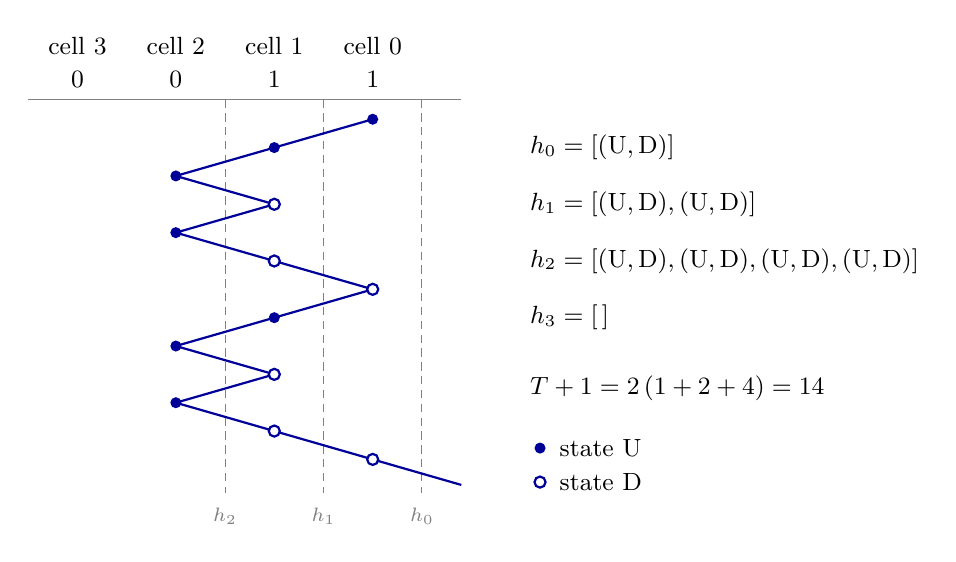
\begin{tikzpicture}[x=1.25cm,y=0.36cm]
  \foreach \c/\b in {0/1,1/1,2/0,3/0} {
    \node[font=\small] at (-\c,1.6) {cell \c};
    \node[font=\small] at (-\c,0.4) {\b};
  }
  \draw[gray] (-3.5,-0.3) -- (0.9,-0.3);
  \foreach \i in {0,1,2} {
    \draw[densely dashed,gray] (-\i+0.5,-0.3) -- (-\i+0.5,-14.2);
  }
  \draw[thick,blue!60!black] (0,-1) -- (-1,-2) -- (-2,-3) -- (-1,-4) -- (-2,-5) -- (-1,-6) -- (0,-7) -- (-1,-8) -- (-2,-9) -- (-1,-10) -- (-2,-11) -- (-1,-12) -- (0,-13) -- (0.9,-13.9);
  \fill[blue!60!black] (0,-1) circle (2pt);
  \fill[blue!60!black] (-1,-2) circle (2pt);
  \fill[blue!60!black] (-2,-3) circle (2pt);
  \draw[blue!60!black,fill=white,thick] (-1,-4) circle (2pt);
  \fill[blue!60!black] (-2,-5) circle (2pt);
  \draw[blue!60!black,fill=white,thick] (-1,-6) circle (2pt);
  \draw[blue!60!black,fill=white,thick] (0,-7) circle (2pt);
  \fill[blue!60!black] (-1,-8) circle (2pt);
  \fill[blue!60!black] (-2,-9) circle (2pt);
  \draw[blue!60!black,fill=white,thick] (-1,-10) circle (2pt);
  \fill[blue!60!black] (-2,-11) circle (2pt);
  \draw[blue!60!black,fill=white,thick] (-1,-12) circle (2pt);
  \draw[blue!60!black,fill=white,thick] (0,-13) circle (2pt);
  \node[font=\scriptsize,gray] at (0.5,-15) {$h_0$};
  \node[font=\scriptsize,gray] at (-0.5,-15) {$h_1$};
  \node[font=\scriptsize,gray] at (-1.5,-15) {$h_2$};
  \node[font=\small,anchor=west] at (1.5,-2) {$h_0=[(\U,\D)]$};
  \node[font=\small,anchor=west] at (1.5,-4) {$h_1=[(\U,\D),(\U,\D)]$};
  \node[font=\small,anchor=west] at (1.5,-6) {$h_2=[(\U,\D),(\U,\D),(\U,\D),(\U,\D)]$};
  \node[font=\small,anchor=west] at (1.5,-8) {$h_3=[\,]$};
  \node[font=\small,anchor=west] at (1.5,-10.5) {$T+1=2\,(1+2+4)=14$};
  \fill[blue!60!black] (1.7,-12.6) circle (2pt); \node[font=\small,anchor=west] at (1.8,-12.6) {state $\U$};
  \draw[blue!60!black,fill=white,thick] (1.7,-13.8) circle (2pt); \node[font=\small,anchor=west] at (1.8,-13.8) {state $\D$};
\end{tikzpicture}
\caption{Machine $378$ on the input $3$ (time runs downwards, $13$ steps; a dot shows the position and the
state of the head before a step). The dashed lines are the cell boundaries with their crossing sequences:
every pair corresponds to one crossing to the left and the next crossing back to the right.}
\label{fig:cross}
\end{figure}

\section{Certificates}\label{sec:cert}

\subsection{The automaton}
Let $\Sigma=\{\U,\D\}^2$ be the set of pairs. A certificate contains a deterministic finite automaton
$(Q,q_0,\delta)$ over $\Sigma$; for a history $h$ we write $q(h)$ for the state reached from $q_0$. In all
certificates used here the state records the whole history as long as it has at most $J$ entries, and
afterwards its first $J$ and its last $j$ entries, with $J\le2$ and $j\le1$; the automaton therefore has at
most $85$ states. Each state $q$ carries a number $\mathit{lo}(q)$ and a flag $\mathit{ex}(q)$ such that every
history $h$ with $q(h)=q$ has length at least $\mathit{lo}(q)$, and exactly $\mathit{lo}(q)$ if the flag is
set. A set $A\subseteq Q\times\Sigma$ of \emph{allowed transitions} defines a language: $h$ is
\emph{$A$-accepted} if the run of the automaton on $h$ uses transitions in $A$ only.

\subsection{Two invariants}
The input region (cells that may hold either symbol) and the blank region (cells $n,n+1,\dots$ of an input
$x<2^n$, all zero) are treated separately but in the same way. For each of them the certificate contains two
sets of allowed transitions, $A_{\mathrm D}$ and $A_{\mathrm G}$, with the following meaning.

\begin{itemize}[leftmargin=2em]
\item \emph{Forward invariant} (Lean: \lean{FwdInv}). Every history of a session on a tape part of the region
is $A_{\mathrm D}$-accepted. This expresses what a tape part can answer at all, whatever is asked of it; for
instance, it may exclude that a call entered in state $\D$ returns in state $\U$.
\item \emph{Top-down invariant with weights} (Lean: \lean{TdInv}). If $h$ is $A_{\mathrm G}$-accepted, $h'$ is
$A_{\mathrm D}$-accepted and $\operatorname{Compat}(b;\,h,h';\,b')$ holds for a symbol $b$ of the region, then
$h'$ is $A_{\mathrm G}$-accepted and
\begin{equation}\label{eq:growth}
\len{h'}\;\le\; \lambda\,\len{h}+\Delta\bigl(b,q(h),q(h')\bigr),
\end{equation}
where the \emph{growth factor} $\lambda\in\{1,2\}$ is fixed for the machine and $\Delta$ is a table of integers contained in the certificate
(only for the triples that can occur).
\end{itemize}
The checker also tests that the initial history $[(\U,r)]$ is $A_{\mathrm G}$-accepted whenever it is
$A_{\mathrm D}$-accepted, and that at the border between the two regions acceptance carries over from the
tables of the input region to those of the blank region. Hence all histories $h_i$ of a halting run are
$A_{\mathrm G}$-accepted, and consecutive ones satisfy~\eqref{eq:growth}.

Both invariants are established by finite \emph{product invariants}, which is what the certificate actually
stores and what the checker tests. A product state describes one cell while it processes a history: its
current symbol, the state of the automaton after the part of $h$ processed so far, the state of the automaton
after the part of $h'$ produced so far and, while a call is in progress, the entry state or required exit
state and the current machine state. For the forward invariant the certificate lists a set of product states
that contains the initial ones and is closed under the moves of the cell, where an excursion to the left may
return in any state permitted by $A_{\mathrm D}$ for the rest of the tape; soundness follows by induction on
the cost of the session, because the session on the rest of the tape is shorter. For the top-down invariant
each product state additionally carries an integer potential $\pi$ such that starting a new entry of $h$
lowers $\pi$ by at most $\lambda$ and every excursion raises it by at least $1$; then $\len{h'}-\lambda\,\len{h}$ is
bounded by the potential at the end, which is bounded by $\Delta$. Product states from which the cell can
never be left in the required state are marked as \emph{dead} and need no potential; this matters because a
cell cannot know in advance in which state the rest of the tape will return the head. The search program
obtains the sets as least fixed points and the potentials as longest-path distances.

\subsection{Potentials for the one-counter system}
After this step, a machine is abstracted to a system whose configurations are pairs $(q,\ell)$ of an automaton
state and a length, with a transition $(q,\ell)\to(q',\ell')$ whenever $\Delta(b,q,q')$ is defined for some
$b$ and $\ell'\le \lambda\ell+\Delta(b,q,q')$. By~\eqref{eq:time} it remains to bound the sum of the lengths along
every path of this system that starts in $(q([(\U,r)]),1)$ and makes at most $n$ transitions in the input
region followed by transitions in the blank region. This is done by potential functions
$W_{\mathrm{in}}(q,\ell,k)$ ($k$ = number of remaining input cells) and $W_{\mathrm{bl}}(q,\ell)$ and a
positive integer scaling factor $d$ such that, for all admissible lengths,
\begin{align*}
d\cdot 2\ell+W_{\mathrm{in}}(q',\ell',k)&\le W_{\mathrm{in}}(q,\ell,k+1), &
d\cdot 2\ell+W_{\mathrm{bl}}(q',\ell')&\le W_{\mathrm{bl}}(q,\ell),\\
W_{\mathrm{bl}}(q,\ell)&\le W_{\mathrm{in}}(q,\ell,0), &
W_{\mathrm{in}}(q_0,0,k)\ge0,\ \ &W_{\mathrm{bl}}(q_0,0)\ge0,
\end{align*}
along every transition. By induction on the remaining cells and the cost (Lean: \lean{AbsSys.boundI},
\lean{boundB}) every session with an $A_{\mathrm G}$-accepted history $h$ and cost $c$ on a tape part that is
blank from its $k$-th cell on satisfies $d\,(c+\len{h})\le W_{\mathrm{in}}(q(h),\len{h},k)$. For a halting run on
an input $x<2^n$ this gives
\[ d\,(T+1)\;\le\; W_{\mathrm{in}}\bigl(q([(\U,r)]),1,n\bigr). \]

Two shapes of potentials are used. For $\lambda=1$ each $W(q,\cdot,\cdot)$ is a polynomial of degree at most two in
$\ell$ and $k$ with integer coefficients, and the certificate is accepted only if
$W_{\mathrm{in}}(q,1,n)\le d\cdot2(n+2)^2$ for the possible initial states $q$ and all $n\ge1$; this yields
$T+1\le2(n+2)^2$ (Lean: \lean{Cert.sound}). For $\lambda=2$ the potentials have the form
$(\alpha\ell+\gamma)2^k+\beta\ell+\delta$, the final condition is $W_{\mathrm{in}}(q,1,n)\le d\,(2^{n+2}-2)$, and
the result is $T+3\le2^{n+2}$ (Lean: \lean{CertE.sound}). The inequalities between potentials are universally
quantified over $\ell,\ell',k$; the checker replaces them by sufficient conditions on the coefficients: after
the substitution $\ell=\ell_0+u$ with the smallest admissible $\ell_0$, and using monotonicity in $\ell'$, the
difference of the two sides must be a polynomial in $u$ and $k$ (respectively an expression
$(A_0+A_1u)2^k+B_0+B_1u$) whose coefficients satisfy sign conditions that imply non-negativity for all
$u,k\ge0$.

\subsection{The checker and the certificates}
The checker is a Boolean function \lean{Cert.check} (respectively \lean{CertE.check}) on the finite tables of
a certificate, and the soundness theorems state that a certificate that passes for machine $m$ implies the
bound for every halting run of $m$ on every input $x<2^n$, $n\ge1$. Each of the $4092$ certificates is then
accepted by a proof of the form \lean{c.check m = true := by decide +kernel}, i.e.\ by evaluating the checker
inside the Lean kernel. The search program (Python, with a linear-programming solver for the potentials) is
not part of the trusted base: a wrong certificate would simply be rejected.

\begin{table}[h]
\centering\small
\begin{tabular}{lr}
\toprule
treatment & machines\\
\midrule
certificate with quadratic potentials ($\lambda=1$), bound $T\le 2(n+2)^2-1$ & 4084\\
certificate with exponential potentials ($\lambda=2$), bound $T\le 2^{n+2}-3$ & 8\\
individual proof (Section~\ref{sec:special}) & 4\\
\bottomrule
\end{tabular}

\medskip
\begin{tabular}{lr}
\toprule
automaton $(J,j)$ & machines\\
\midrule
$(0,0)$ & 3595\\
$(1,0)$ & 448\\
$(1,1)$ & 41\\
$(2,0)$, $(2,1)$ & 8\\
\bottomrule
\end{tabular}
\caption{How the $4096$ machines are covered, and the automata used by the $4092$ certificates.}
\label{tab:stats}
\end{table}

The eight machines with $\lambda=2$ are $378$, $924$, $1351$, $1953$, $2142$, $2289$, $3626$ and $3717$; their
histories can double from one cell to the next, as in Figure~\ref{fig:cross}. For most machines the automaton
has only two states, and the tables are small (about $43$ product states on average, at most $801$);
the scaling factor $d$ is $1$ for $4001$ machines and at most $18$. The bound for a machine with $\lambda=1$ is at
most the conjectured value for every $n$, because $2(n+2)^2+2\le2^{n+2}$ for $n\ge5$; the bound for a machine
with $\lambda=2$ is at most the conjectured value because $2^{n+2}-3\le2(n+2)^2-1$ for $1\le n\le4$.

\section{The four remaining machines}\label{sec:special}

For the machines $1507$ and $3555$, and for $2574$ and $2830$, whose rules are obtained from those of the first
two by exchanging the symbols $0$ and $1$ (the blank tape, of course, still consists of zeros), the scheme of Section~\ref{sec:cert} fails
for every automaton that was tried: a single visit of a cell can involve arbitrarily many excursions to the
left, so no bound of the form~\eqref{eq:growth} with finitely many classes was found. Their behaviour is
nevertheless simple (file \lean{A393317/Special.lean}).

Consider $1507$ and $3555$. Both have the rules $\D1\to\D0\mathrm{L}$, $\D0\to\U1\mathrm{R}$ and
$\U0\to\D1\mathrm{R}$. Suppose the head is in state $\D$ on cell $r$, with ones on the cells $r,\dots,r+d-1$ and a
zero on cell $r+d$. The head sweeps left and erases the $d$ ones; on the zero it turns; on the way back the
two rules for the symbol $0$ write the ones again, changing the state at each step, like a zip. After $2d+1$
steps the head leaves cell $r$ to the right, in state $\U$ if $d$ is even and in state $\D$ if $d$ is odd, and
the only change on the tape is a new one on cell $r+d$ (Lean: \lean{FamA.dev}). One shows that, in a run that does not halt with its first step, the cells to the right of the first zero
always form a solid block of ones; each event consumes one zero and takes a number of steps that is linear in
the length of the block. What differs between the two machines is the behaviour of
state $\U$ on a one ($1507$ walks left to the first zero, $3555$ switches to state $\D$), and one has to treat
the input region, where zeros are followed by further ones, and the blank region, where a run either comes
back to cell $0$ through a chain of events or never halts. The results are
\[ T\le 4n^2 \ \ (1507,\ n\ge2),\qquad T\le 7\ \ (1507,\ n=1),\qquad T\le 2n^2+4n+7\ \ (3555) \]
for every halting run on an input $x<2^n$. The machines $2574$ and $2830$ have the mirrored rules
$\D0\to\D1\mathrm{L}$, $\D1\to\U0\mathrm{R}$, $\U1\to\D0\mathrm{R}$; here the events sweep over zeros and consume
ones, a head in state $\D$ on a part of the tape without ones never returns, and $T\le4n^2$ for $n\ge1$. All
these bounds are at most the conjectured value: $4n^2\le2(n+2)^2-1$ for $n\le4$, $4n^2+3\le2^{n+2}$ for $n\ge5$,
and $2n^2+4n+7\le2(n+2)^2-1$ for all $n$.

\section{The formal statements and how to check them}\label{sec:formal}

The statements of Theorem~\ref{thm:main} in Lean are as follows (file \lean{Challenge.lean}, which contains the
model and these two statements and nothing else).

{\footnotesize
\begin{verbatim}
def haltingTimes (n : ℕ) : Set ℕ :=
  {t | ∃ m < 4096, ∃ x, 2 ^ (n - 1) ≤ x ∧ x < 2 ^ n ∧ HaltsAfter m (init x) t}

def haltingTimesUpTo (n : ℕ) : Set ℕ :=
  {t | ∃ m < 4096, ∃ x, x < 2 ^ n ∧ HaltsAfter m (init x) t}

theorem hasler_conjecture (n : ℕ) (hn : 1 ≤ n) :
    IsGreatest (haltingTimes n) (if n < 5 then 2 * (n + 2) ^ 2 - 1 else 2 ^ (n + 2) - 3)

theorem hasler_conjecture_upto (n : ℕ) (hn : 1 ≤ n) :
    IsGreatest (haltingTimesUpTo n) (if n < 5 then 2 * (n + 2) ^ 2 - 1 else 2 ^ (n + 2) - 3)
\end{verbatim}
}

\noindent Theorem~\ref{thm:single} corresponds to the theorems \lean{machine378}, \lean{machine1351} and
\lean{machine1447} in the file \lean{A393317/Stage1.lean} and to \lean{max378}, \lean{max1351} and
\lean{max1447} in the file \lean{A393317/Main.lean}.

The repository is a self-contained Lake project (Lean v4.27.0, Mathlib v4.27.0). Running
\lean{lake exe cache get} and \lean{lake build} compiles everything, including the $4092$ certificate checks
and the comparison with the OEIS data, and prints the axioms used by the main theorems; on a machine with $16$
cores this takes about seven minutes. Independently of the build, the statements can be checked with
Comparator~\cite{comparator}, which verifies that the theorems named in \lean{comparator.json} are proved in
\lean{Solution.lean} with exactly the statements and definitions of \lean{Challenge.lean}, replays the proof in
the Lean kernel and checks the list of axioms. The hand-written part of the development has about $3100$
lines; the generated certificates take about $9$\,MB.

\section{Status of this work and authorship}\label{sec:status}

\subsection*{Authorship}
The choice of the problem, the proof and its formalization in Lean were produced by Claude Fable~5, an AI
model made by Anthropic (model ID \texttt{claude-fable-5-2}, working in Claude Code), on 10~November 2026;
this text was written by the same model. The work was commissioned by Dr.~Marc Potempa, who set the task
(to find an open problem, to solve it and to have the solution verified by a proof checker) and decided to
publish the result, but did not contribute to the mathematical content.

\subsection*{What has and has not been checked}
\begin{itemize}[leftmargin=2em]
\item The proofs are checked by the Lean kernel and by Comparator. They were checked with the standard Lean
kernel only; no second, independent kernel has been used.
\item No human has read the proof or this description. The description is meant as a guide to the formal
development; where the two differ, the Lean files are authoritative.
\item The definition of the model (file \lean{A393317/Defs.lean}; the file \lean{Challenge.lean} repeats
it) was written by the AI model and does not come from an external source. It has been
tested against published data as described in Remark~\ref{rem:validation}, but no second person has reviewed
it. Should it deviate from Wolfram's set-up in a way that these tests do not detect, the theorems would remain
true statements, but about a slightly different model.
\item The search for earlier proofs was done with the means described in the introduction and may be
incomplete.
\end{itemize}

\begin{thebibliography}{9}
\bibitem{oeis} OEIS Foundation Inc., \emph{The On-Line Encyclopedia of Integer Sequences}, entry A393317
(S.~A.~Irvine, 10 Feb 2026; conjecture by M.~F.~Hasler, 12 Feb 2026; further terms and program by
R.~P.~P.~McKone), \url{https://oeis.org/A393317}. Related entries: A392245, A393103, A393106, A393146, A393190,
A393209, A393210, A393212, A393232, A393233, A393234.
\bibitem{wolfram} S.~Wolfram, \emph{P vs.\ NP and the Difficulty of Computation: A Ruliological Approach},
Stephen Wolfram Writings, January 2026,
\url{https://writings.stephenwolfram.com/2026/01/p-vs-np-and-the-difficulty-of-computation-a-ruliological-approach/}.
\bibitem{hennie} F.~C.~Hennie, \emph{One-tape, off-line Turing machine computations}, Information and Control
\textbf{8} (1965), 553--578.
\bibitem{bb5} The bbchallenge Collaboration, \emph{Determination of the fifth Busy Beaver value},
arXiv:2509.12337.
\bibitem{lean4} L.~de Moura and S.~Ullrich, \emph{The Lean 4 theorem prover and programming language},
in: Automated Deduction -- CADE 28, Lecture Notes in Computer Science 12699, Springer, 2021, 625--635.
\bibitem{mathlib} The mathlib Community, \emph{The Lean mathematical library}, in: Proceedings of the 9th ACM
SIGPLAN International Conference on Certified Programs and Proofs (CPP 2020), 367--381.
\bibitem{comparator} \emph{Comparator}, a tool for checking Lean proofs against a given statement,
\url{https://github.com/leanprover/comparator}.
\bibitem{trureturing} GitHub repository \texttt{the-omega-institute/trureturing}, pull request 25879,
\emph{formalize: prove Bala's exact halting formula for machine 3626}, November 2026,
\url{https://github.com/the-omega-institute/trureturing/pull/25879}.
\end{thebibliography}

\end{document}
